\section{Pésentation}
\vspace{0.6cm}

\subsection{Le sujet}
Dans ce projet nous devrons réaliser un code visant à aider Homer à trouver le chemin le plus court vers les donuts en
évitant les ennemis. C'est-à-dire nous devrons créer un environnement, des actions et des récompenses en fonction de la position dans l'environnement. Pour cela, nous devrons utiliser le processus de décision markovien et ainsi prendre en compte une part d'aléatoire dans les décisions de l'agent.
\vspace{0.6cm}

\FloatBarrier %bloque l'image dans le texte
\begin{figure}[!h]
\centering
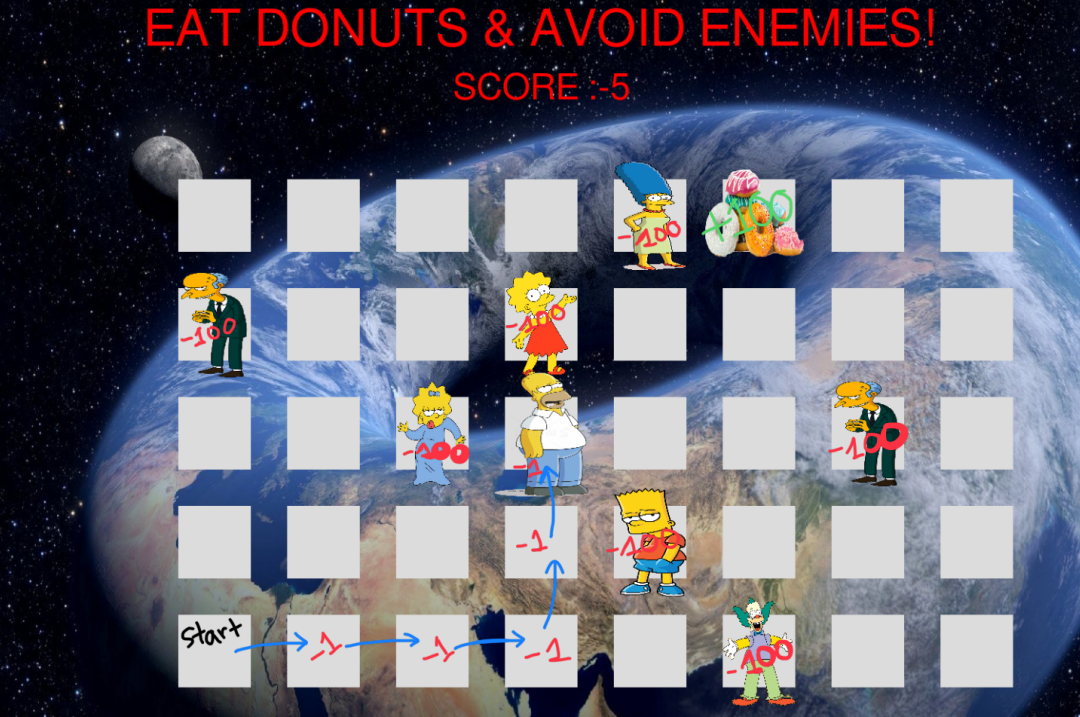
\includegraphics[width=14cm,scale=1]{Capture2.PNG}
\caption{Exemple de l'interface à obtenir}
\end{figure}
\FloatBarrier


\subsection{Problème soulevé}

D'abord, ce sujet nous laisse relativement libre et afin de commencer au mieux, notre encadrante nous a proposé des mots clés pour savoir dans quelle direction partir : 
\begin{itemize}
  \item[$\bullet$] programmation dynamique (itération de politique, itération de valeur) ;
  \item[$\bullet$] apprentissage par renforcement ; 
  \item[$\bullet$] environnement stochastique ;
  \item[$\bullet$] model based / model free ; 
  \item[$\bullet$] processus décisionnel Markovien.
\end{itemize}


Cela permet de mieux comprendre le sujet et nous guider vers ce que nous devons faire dans la suite.


\subsubsection{Programmation dynamique}
 La programmation dynamique consiste à résoudre un problème en le décomposant en sous-problèmes, puis à résoudre les sous-problèmes, des plus petits aux plus grands en stockant les résultats intermédiaires.
 
\subsubsection{Apprentissage par renforcement}

L'apprentissage par renforcement est une méthode utilisée pour créer des intelligences artificielles. On appelle \textbf{agent autonome} la machine (robot ou autre) à qui on fait subir cet apprentissage. Grâce à des expériences répétées un grand nombre de fois, l'agent cherche à maximiser la récompense qui lui est attribuée quand il réussit la tâche que l'on veut qu'il effectue.

\subsubsection{Environnement stochastique}
Un environnement stochastique est un environnement dont les paramètres évoluent de manière aléatoire. Cela s’oppose aux environnements dits déterministes. Les organismes vivant dans ces habitats variables et imprévisibles doivent donc s’adapter rapidement afin d’y survivre et de pouvoir s’y reproduire. (\href{https://fr.wikiversity.org/wiki/Adaptations_aux_environnements_stochastiques#:~:text=Un\%20environnement\%20stochastique\%20est\%20un,de\%20pouvoir\%20s'y\%20reproduire.}{Wikipédia})

\subsubsection{Modèle}
Un modèle est un environnement dans lequel un agent évolue. On sépare habituellement deux manières d'effectuer un apprentissage, désignés par les termes anglais : model based et model free.
\begin{enumerate}
\item{\underline{Model based}}\\
Dans une simulation dite "model based", l'agent peut "demander" à l'environnement quelles récompenses il obtiendra si il fait telle ou telle action, lui permettant de prédire son futur score. Pour trouver le chemin optimal, il peut donc tenter d'améliorer le plus possible son chemin pendant l'éxécution du programme.
\item{\underline{Model free}}\\
Dans une simulation dite "model free", l'agent évolue à l'aveugle et ne connait la récompense d'une action que quand il l'effectue. Pour trouver le chemin optimal, il doit donc effectuer un grand nombre de répétitions de l'expérience avant d'avoir des données suffisantes pour pouvoir savoir où aller. Ce genre de modèles n'est régi que par l'aléatoire, contrairement au précédent.
\end{enumerate}

\subsubsection{Processus décisionnel Markovien}

Dans notre projet, l'objectif sera d'entraîner un modèle afin qu'à l'issue de l'entraînement, Homer trouve le plus court chemin jusqu'aux donuts et ainsi que le problème soit résolu.

Il existe différents types d'apprentissage afin d'entraîner notre modèle. \\
Mais tout d'abord il faut modéliser le problème et pour cela nous allons utiliser un processus décisionnel markovien (MDP). Un MDP est un quadruplet \{ S , A , T , R \} qui définit : 
\begin{itemize}
  \item[$\bullet$] \textbf{S} : qui représente l'ensemble les états d'un environnement ;
  \item[$\bullet$] \textbf{A} : l'ensemble des actions applicable dans notre environnement à savoir les déplacements de Homer d'une case à l'autre (haut, bas, droite, gauche) ; 
  \item[$\bullet$] \textbf{T} : la fonction probabilité de transition qui définis la probabilité que Homer passe d'un état à un autre en fonction de l'action appliqué ;
  \item[$\bullet$] \textbf{R} : la fonction qui associe chaque état de l'environnement à une récompense (case vide : SCORE - 1, case avec ennemi :  SCORE - 100, case avec donuts  : SCORE + 100).
\end{itemize}
